\documentclass[a4paper, 11 pt]{article}
\input{General/Preamble} % Loads in the preamble 
\input{General/Settings} % Loads in user defined settings
\input{General/MathCommands} % Loads in user defined math commands

\begin{document}

%%% PAGE DE GARDE
\thispagestyle{empty}
\begin{center}
    \newcommand{\HRule}{\rule{\linewidth}{0.5mm}}
    
    \textsc{\LARGE École Polytechnique Fédérale de Lausanne}\\[0.5cm]
    
\includegraphics[width=5cm]{Figures/epfl_red.png}\\[0.5cm]
    \LARGE{\textsc{Robotique, 2025-26}}\\[0.5cm]
    \huge{\textbf{Semester Project}}
    
    \HRule \\[0.4cm]
    {\huge \bfseries Textometric analysis of Swiss spatial planning policies}\\[0.1cm]
    \HRule \\[0.5cm]
    \LARGE{\textsc{Urban Sociology Laboratory} \\
    \text{27.08.2025 - 12.12.2025}}\\[0.5cm]
    
    \vspace{5mm}
    %\includegraphics[scale=0.6]{images/pageDeGarde.png}\\
    \vspace{15mm}
    
    \begin{minipage}{2in} \Large
    \textbf{Author:}\\
    Nathann \textsc{Morand}\\
    Robotics M.Sc.
    \end{minipage}
    \hfill
    \begin{minipage}{2.5in} \Large
    \textbf{Supervisors:}\\
    Prof. Vincent \textsc{Kaufmann} \\
    Jules \textsc{Grandvillemin} \\
    \end{minipage}
\end{center}
%%%

%%% ABSTRACT, PROJECT ASSIGNMENT
{ % create local environment
\fancyhead[R]{\textsc{PROJECT ASSIGNMENT, ABSTRACT}}

\newpage
\section*{Abstract}
\addcontentsline{toc}{section}{Abstract}
This study investigates how accessibility, motility, and time are represented in Swiss spatial planning discourse through a textometric approach.\\ It does so using a corpus made of 74 plans accross all cantons of switzerland spanning between 1987 to 2025.
The results reveal a pronounced imbalance: accessibility dominates and is expressed in concrete, operational terms, while the other aspect of motility,  skills, motivation, and cognitive appropriation is almost entirely absent. This absence shows that capability-based understandings of mobility remain outside the institutional vocabulary.\\
Time-related notions display a similar asymmetry. Objective and measurable aspects of time are frequently mentioned, whereas perceived or subjective time appears only marginally. Concepts such as comfort are present but vaguely defined, suggesting that experiential dimensions of mobility are acknowledged but not yet integrated into planning practice.

The textometric method proved effective in exposing what institutional discourse emphasizes and what it leaves unspoken. Furthermore, this approach, while not perfect, reduce researcher bias by offering some quantitative result.\\
The project contributes both by offering an analysis that show a discursive bias toward technical framings of mobility and an open, dataset with a CC-BY license to support further research.\\
Overall, the findings underline the need for conceptual and institutional shifts to incorporate motility and experiential time into planning. Doing so would help move Swiss mobility policy toward mobility policies that better account for citizen capabilities and experiential aspects of travel, and thus help transition to a more sustainable mobility.

\newpage
}
%%%
%%% TABLE OF CONTENTS
\newpage
\renewcommand{\contentsname}{Table of Contents} 
{
  \hypersetup{linkcolor=black}
  \tableofcontents
}
\newpage
%%%

% Creates the introduction, starting page numbering
\section{Introduction}

\subsection{Background: Spatial Planning and Transport Policies in Switzerland}
Spatial planning in Switzerland operates in a layered fashion.
The federal Spatial Planning Act (LAT: Loi sur l'aménagement du territoire) \cite{noauthor_rs_nodate} was introduced in 1979 by the Confederation and apply to each Cantons and Communes.
It defines the overall framework and general objectives such as containing urban sprawl, protecting natural resources, and ensuring efficient land use, but delegates the implementation to the Cantons. Each Canton is responsible for elaborating a "cantonal master plan" (plan directeur cantonal) within the first eight years of the LAT’s introduction and then revising it at least every ten years. The Confederation must review and approve each plan and its revisions.  

These plans translate federal principles into territorial strategies that account for local geography and specific needs. Once approved by the Confederation, they become binding for public authorities but remain indicative for private actors, shaping how subsequent zoning and land-use decisions are made. The Cantons delegate the responsibility for implementing the measures to the Communes, with the exception of cantonal infrastructure such as cantonal roads, which remain under cantonal responsibility.  

The Communes achieve the goals either by adopting local regulations (règlement communal) or by directly implementing measures, for instance by creating new bike lanes. Some Communes also prepare a "local master plan" (plan d’affectation communal), which materializes these strategies by determining the precise allocation of land and the regulations governing its use.  

This nested structure creates offer flexibility to adapt the general goal as close as possible to the local reality but it require a fair amount of effort to ensure the efficient communication between all the actors. Over time, revisions of the LAT, most notably in 2014 \cite{ssemblee_federale_de_la_confederation_suisse_ro_2014}, shifted the discourse from expansion toward densification, sustainability, and the coordination of land use with transport systems. The vast majority of early plans exist only as paper archives available only trough physical consultation, limiting historical analysis, but comparative studies between cantonal documents remain meaningful. Each plan reveals how spatial and transport policies adapt a shared legal foundation to diverse territorial realities and political cultures.

\newpage

\subsection{Research Motivation: Linking Travel Behavior, Planning, and Text Analysis}

Effective policy design requires a systemic perspective. Interventions that optimize without taking into account the system as a whole often if not always generate unintended consequences\cite{merton_unanticipated_1936}. The problem is actually very similar to what arise in artificial intelligence when systems end up acting in unanticipated ways due to failure (among other factor) of the cost function to capture the entirety of the human intent with the only goal of minimize the said cost function \cite{maier_take_2025}.

his principle directly applies to transportation policy. One of its main goals is to reduce environmental harm by lowering greenhouse gas emissions, which are the primary cause of human-induced climate change. The transport sector plays a key role in this effort. In Europe, it is the only major sector where emissions have not decreased, and it remains the second-largest emitter after energy production \cite{noauthor_co2_2019}. Decarbonizing transport is therefore essential for mitigating climate change. However, greenhouse gases are not the only negative externality. Transport also generates tire-related microplastics, fine particles, noise pollution, accident risks, soil sealing, and barriers to animal movement. These impacts must be balanced with other objectives derived from the right to mobility \cite{nations_universal_nodate}, such as equity and inclusivity, economic efficiency, and safety. Ultimately, transport policy must navigate a tradeoff between protecting the environment and its inhabitants from harmful externalities and ensuring the human need for mobility.

A transition to active mobility and public transport offers the most equitable path forward. Private vehicles are highly inefficient in their use of urban space. They provide primary benefits to a minority of users. This often occurs at a significant cost to the broader community \cite{litman_evaluating_2007}. Prioritizing sustainable modes is a matter of fairness and justice \cite{guo_case_nodate}.

However, the existence of sustainable infrastructure does not guarantee its use. Research, such as the work of J. Grandvillemin, demonstrates this clearly. Modal choice is not a purely rational decision. It is shaped by intangible factors like personal habits, preferences, and perceived access. The sociological concept of motility effectively captures this capacity for mobility \cite{kaufmann_motility_2004}. Understanding these human factors is crucial for designing effective systems.

This leads to the core research question of this document. To what degree are these human dimensions of mobility integrated into Swiss spatial planning? This study investigates whether cantonal master plans consider the factors that truly shape travel behavior. It aims to determine if planning discourse addresses how people experience time and choose between mobility options. The ultimate goal is to assess if Swiss policy aligns physical infrastructure with the human elements of mobility.
\subsection{Research Questions}

To what extent do Swiss territorial / spatial planning documents acknowledge the distinction between perceived time vs measured/travel-time objectively modeled, in relation to modal choice?

How strongly do Swiss planning documents incorporate human / behavioral / motility-based rationales, as opposed to purely economic / efficiency rationales, in shaping transport and spatial policy?
 
\include{Chapters/ch2}
\section{State of the Art}
Traditional conceptions of mobility were primarily based on metrics that fail to capture all the factors at play. The work of Geurs and van Wee \cite{geurs_accessibility_2004} provides a comprehensive review of accessibility measures. They identified a gap in operational planning methods, which tend to be overly reductionist by using metrics such as travel speed or congestion level to facilitate the interpretation and communication of results. They showed that the quality and theoretical soundness of such evaluations could be greatly improved by taking into account behavioral and spatial dimensions, as well as the feedback loops that shape mobility, but their framework still does not account for the lived experience of travel.\\

This is where sociological approaches, from Sheller and Urry \cite{sheller_new_2006} and more notably Kaufmann's concept of motility \cite{kaufmann_motility_2004} and Doherty's notion of viscosity \cite{doherty_agentive_2015}, shine by providing a theoretical framework to explain the mismatch between predicted theoretical outcomes and observed results. Their work emphasizes how individuals experience travel and how their choices are shaped by these experiences. Jain and Lyons \cite{jain_gift_2008} further contribute to this through their research “The Gift of Travel Time,” by challenging the idea that travel time is purely a waste and should therefore be minimized. They demonstrate how individuals can re-appropriate this time for meaningful activities, making perceived time fundamentally different from measured time. This distinction shows that the quality of the journey matters at least as much as its speed. Bühler \cite{buhler_habit_2020} extends this perspective by noting the importance of habits and routines in modal choice, illustrating how decision-making is not purely rational but embedded in social and temporal practices.\\

Together, these works depict a more complete image of mobility through, first, the classical approach, which models accessibility as a measurable property, and second, the sociological approach, which presents mobility as a lived and experienced process.\\

The present study aims to assess how far these theoretical concepts have made their way into operational planning by analyzing a corpus of Swiss spatial policy documents, in order to determine whether planning discourse reflects a human-centered understanding of mobility or remains anchored in purely functional and physical-based reasoning. To do so, a total of fourty word where selected from the vocabulary present in theses publication and through exploration of the corpus and then mapped to a concept. With a few words per concept we can start to measure how much a concept is present in a text corpus as theorized in the textometric approach.\\
\section{Methodology}


I manually downloaded the PDF on each canton's website.
{\footnotesize
\setlength{\tabcolsep}{3pt}
\renewcommand{\arraystretch}{1.1}

\begin{minipage}[t]{0.49\textwidth}
\centering

% === First half of table ===
\begin{longtable}{|p{1cm}|p{1cm}|p{1.5cm}|p{1.5cm}|p{1cm}|}
\hline
\rotatebox{70}{\textbf{Canton}} &
\rotatebox{70}{\textbf{Version}} &
\rotatebox{70}{\textbf{Year}} &
\rotatebox{70}{\textbf{Availability}} &
\rotatebox{70}{\textbf{Language}} \\ 
\hline

\multirow{3}{*}{AG} & 3 & 2025 & \href{https://www.ag.ch/de/themen/planen-bauen/raumentwicklung/grundlagen-und-kantonalplanung/richtplan}{Online} & DE \\
 & 2 &  & † & DE \\
 & 1 &  & ‡ & DE \\ \hline

\multirow{3}{*}{AR} & 3 & 2025 & \href{https://ar.ch/verwaltung/departement-bau-und-volkswirtschaft/amt-fuer-raum-und-wald/abteilung-raumentwicklung/planen/kantonale-planung/}{Online} & DE \\
 & 2 &  & † & DE \\
 & 1 &  & ‡ & DE \\ \hline

\multirow{3}{*}{AI} & 3 & 2018 & \href{https://www.ai.ch/themen/planen-und-bauen/raumplanung/richtplanung}{Online} & DE \\
 & 2 &  & † & DE \\
 & 1 &  & ‡ & DE \\ \hline

\multirow{3}{*}{BE} & 3 & 2024 & \href{https://www.raumplanung.dij.be.ch/fr/start/kantonaler-richtplan.html}{Online} & DE \\
 & 2 &  & † & DE \\
 & 1 &  & ‡ & DE \\ \hline

\multirow{3}{*}{BL} & 3 & 2009 & \href{https://www.baselland.ch/politik-und-behorden/direktionen/bau-und-umweltschutzdirektion/raumplanung/raumplanung/richtplanung}{Online} & DE \\
 & 2 &  & † & DE \\
 & 1 &  & ‡ & DE \\ \hline

\multirow{3}{*}{BS} & 3 & 2025 & \href{https://www.bs.ch/bvd/staedtebau-architektur/raumplanung/kantonaler-richtplan}{Online} & DE \\
 & 2 &  & † & DE \\
 & 1 &  & ‡ & DE \\ \hline

\multirow{3}{*}{FR} & 3 & 2020 & \href{https://www.fr.ch/dime/seca/plan-directeur-cantonal}{Online} & FR \\
 & 2 &  & † & FR \\
 & 1 &  & ‡ & FR \\ \hline

\multirow{3}{*}{GE} & 3 & 2024 & \href{https://www.ge.ch/dossier/amenager-territoire/planification-cantonale-regionale/plan-directeur-cantonal-2030}{Online} & FR \\
 & 2 &  & † & FR \\
 & 1 &  & ‡ & FR \\ \hline

\multirow{3}{*}{GL} & 3 & 2025 & \href{https://www.gl.ch/verwaltung/bau-und-umwelt/hochbau/raumentwicklung-und-geoinformation/raumentwicklung/kantonale-richtplanung.html/5046}{Online} & DE \\
 & 2 &  & † & DE \\
 & 1 &  & ‡ & DE \\ \hline

\multirow{3}{*}{GR} & 3 & 2025 & \href{https://www.gr.ch/DE/institutionen/verwaltung/dvs/are/dienstleistungen/richtplanung/Seiten/Text-und-Karte.aspx}{Online} & DE \\
 & 2 &  & † & DE \\
 & 1 &  & ‡ & DE \\ \hline

\multirow{3}{*}{JU} & 3 &  & \href{https://www.jura.ch/fr/Autorites/Administration/DEN/SDT/Plan-directeur-cantonal/Plan-directeur-cantonal.html}{Online} & FR \\
 & 2 &  & † & FR \\
 & 1 &  & ‡ & FR \\ \hline

\multirow{3}{*}{LU} & 3 & 2009 & \href{https://richtplan.lu.ch/}{Online} & DE \\
 & 2 &  & † & DE \\
 & 1 &  & ‡ & DE \\ \hline

\multirow{3}{*}{NE} & 3 & 2011 & \href{https://www.ne.ch/autorites/DDTE/SCAT/pdc/Pages/accueil.aspx}{Online} & FR \\
 & 2 &  & † & FR \\
 & 1 &  & ‡ & FR \\ \hline

\caption{Cantonal master plans (part 1).}
\end{longtable}

\end{minipage}
\hfill
\begin{minipage}[t]{0.49\textwidth}
\centering


% === Second half of table ===
\begin{longtable}{|p{1cm}|p{1cm}|p{1.5cm}|p{1.5cm}|p{1cm}|}
\hline
\rotatebox{70}{\textbf{Canton}} &
\rotatebox{70}{\textbf{Version}} &
\rotatebox{70}{\textbf{Year}} &
\rotatebox{70}{\textbf{Availability}} &
\rotatebox{70}{\textbf{Language}} \\ 
\hline

\multirow{3}{*}{NW} & 3 & 2002 & \href{https://www.nw.ch/raumentwdienste/2871}{Online} & DE \\
 & 2 &  & † & DE \\
 & 1 &  & ‡ & DE \\ \hline

\multirow{3}{*}{OW} & 3 & 2019 & \href{https://www.ow.ch/dienstleistungen/1527}{Online} & DE \\
 & 2 &  & † & DE \\
 & 1 &  & ‡ & DE \\ \hline

\multirow{3}{*}{SG} & 3 & 2017 & \href{https://www.sg.ch/bauen/raumentwicklung/kantonaleplanung/richtplanung.html}{Online} & DE \\
 & 2 &  & † & DE \\
 & 1 &  & ‡ & DE \\ \hline

\multirow{3}{*}{SH} & 3 & 2014 & \href{https://sh.ch/CMS/Webseite/Kanton-Schaffhausen/Beh-rde/Verwaltung/Baudepartement/Planungs--und-Naturschutzamt/Raumplanung/Kantonale-Richtplanung-1612737-DE.html}{Online} & DE \\
 & 2 &  & † & DE \\
 & 1 &  & ‡ & DE \\ \hline

\multirow{3}{*}{SZ} & 3 & 2003 & \href{https://www.sz.ch/behoerden/verwaltung/volkswirtschaftsdepartement/amt-fuer-raumentwicklung/kantonaler-richtplan.html/8756-8758-8802-10373-11039-12578}{Online} & DE \\
 & 2 &  & † & DE \\
 & 1 &  & ‡ & DE \\ \hline

\multirow{3}{*}{SO} & 3 & 2017 & \href{https://so.ch/verwaltung/bau-und-justizdepartement/amt-fuer-raumplanung/richtplanung/}{Online} & DE \\
 & 2 &  & † & DE \\
 & 1 &  & ‡ & DE \\ \hline

\multirow{3}{*}{TI} & 3 & 2013 & \href{https://www4.ti.ch/dt/dstm/sst/temi/piano-direttore/piano-direttore/}{Online} & IT \\
 & 2 &  & † & IT \\
 & 1 &  & ‡ & IT \\ \hline

\multirow{3}{*}{TG} & 3 & 2009 & \href{https://raumentwicklung.tg.ch/themen/kantonaler-richtplan.html/4211}{Online} & DE \\
 & 2 &  & † & DE \\
 & 1 &  & ‡ & DE \\ \hline

\multirow{3}{*}{UR} & 3 & 2012 & \href{https://www.ur.ch/dienstleistungen/3687}{Online} & DE \\
 & 2 &  & † & DE \\
 & 1 &  & ‡ & DE \\ \hline

\multirow{3}{*}{VD} & 3 & 2008 & \href{https://www.vd.ch/territoire-et-construction/amenagement-du-territoire/plan-directeur-cantonal/}{Online} & FR \\
 & 2 &  & † & FR \\
 & 1 &  & ‡ & FR \\ \hline

\multirow{3}{*}{VS} & 3 & 2019 & \href{https://www.vs.ch/fr/web/sdt/plan-directeur-cantonal-2019}{Online} & FR \\
 & 2 &  & † & FR \\
 & 1 &  & ‡ & FR \\ \hline

\multirow{3}{*}{ZG} & 3 & 2004 & \href{https://zg.ch/de/planen-bauen/raumplanung/richtplanung#archiv}{Online} & DE \\
 & 2 &  & † & DE \\
 & 1 &  & ‡ & DE \\ \hline

\multirow{3}{*}{ZH} & 3 & 2014 & \href{https://www.zh.ch/de/planen-bauen/raumplanung/richtplaene.html}{Online} & DE \\
 & 2 &  & † & DE \\
 & 1 &  & ‡ & DE \\ \hline

\caption{Cantonal master plans (part 2).}
\end{longtable}

\end{minipage}



\textbf{Legend:}
\begin{itemize}
    \item[†] Only available in paper format (physical consultation) and thus excluded from this study
    \item[‡] Sent upon request by the cantonal service.
\end{itemize}
}





The raw text was extracted from the pdf using a bash one liner

\begin{verbatim}
for f in *.pdf *.PDF; do
  [ -f "$f" ] && pdftotext "$f" "${f%.*}.txt"
done
\end{verbatim}


I then imported the .txt into TXM : https://txm.gitpages.huma-num.fr/textometrie/

TXM use the treetagger module to tag each word in the corpus. (https://www.cis.uni-muenchen.de/~schmid/tools/TreeTagger/) \cite{serge_txm_2010}

I used the French and German module for the French and German dataset.

I used TXM to understand a bit the corpus but in an attempt to make this more reproductible, I translated the useful query into python and made a script to renegerate my result.

I look at hit against a custom keyword list with word mapped to motilité and temps perçu

I did an AFC on the whole corpus to see if there are differences between documents but it did not yield any useful result. the figures are in annexes

I also did an AFC with the hit against time and moitilité
\section{Results}

\subsection{Word Occurences}

In the first table \ref{table:table_motility} The results reveal a strong asymmetry between the two conceptual fields. Terms related to motility are almost absent from both corpora, while accessibility vocabulary is frequent and well represented. This suggests that Swiss spatial planning discourse focuses primarily on infrastructural and material dimensions of mobility. The human, cognitive, and motivational aspects that define motility are not expressed in the language of planning documents. Mobility appears as something provided through networks and infrastructure rather than as a capability that individuals develop and use. The conclusion is the same for French and German.

The same pattern is visible in the analysis of time-related terms in table \ref{table:table_time}. References to physical or objective time largely outweigh those to perceived or subjective time. Travel time is described as a variable to be reduced, optimized, or measured. Few terms evoke comfort or satisfaction. This indicates that time is approached mainly as an operational parameter rather than a human experience. But the contrast is not as dramatic as for motility between the two perspective.

Taken together, these findings show that planning discourse remains centered on measurable, supply-side factors. The subjective dimensions of mobility, including skills, motivation, and perception, are weakly represented not to say absent. The language used in official documents thus reflects and reinforces a narrow view of mobility, oriented toward infrastructure and performance rather than individual capacities and experiences.
\begin{table}[H]
\centering
\caption{Frequency of mobility-related terms in French and German corpora (aligned by conceptual field: Motility vs Accessibility)}
\resizebox{\textwidth}{!}{
\begin{tabular}{@{}llS[table-format=5.0]lS[table-format=5.0]S[table-format=5.0]@{}}
\toprule
\textbf{Category} & \textbf{FR term} & \textbf{FR hits} & \textbf{DE term} & \textbf{DE hits} & \textbf{Total} \\
\midrule
\multicolumn{7}{l}{\textbf{Motility}} \\
\midrule
 & aptitude mobilité & 3 & Bewegungsfähigkeit & 3 & 6 \\
 & capital mobilité & 0 & Mobilitätskapital & 0 & 0  \\
 & habitus mobilité & 0 & Mobilitätshabitus & 0 & 0 \\
 & autonomie déplacement & 0 & Bewegungsautonomie & 0 & 0  \\
 & apprentissage mobilité & 0 & Mobilitätslernen & 0 & 0  \\
 & stratégie déplacement & 1 & Mobilitätsstrategie & 14 & 15  \\
 & compétence & 159 & Orientierungskompetenz & 0 & 159  \\
 & représentation espace & 0 & Raumvorstellung & 0 & 0 \\
 & motivation mobilité & 0 & Mobilitätsmotivation & 0 & 0  \\
 & (valeur) symbolique mobilité & 0 & Symbolisch Mobilität & 0 & 0  \\
\midrule
\textbf{Subtotal (Motility)} &  & 163 &  & 17 & 180 \\
\midrule
\multicolumn{7}{l}{\textbf{Accessibility}} \\
\midrule
 & accessibilité & 284 & Erreichbarkeit & 207 & 491  \\
 & qualité desserte & 159 & Versorgungsqualität & 3 & 162  \\
 & intégration transport & 3 & Verkehrsintegration & 0 & 3  \\
 & coût & 304 & Kosten & 321 & 625 \\
 & disponibilité transport & 1 & Verfügbarkeit verkehrsmittel & 1 & 2 \\
 & infrastructure & 1109 & Infrastruktur & 738 & 1847  \\
 & centralité spatial & 0 & räumlich zentralität & 0 & 0  \\
 & inégalité accès & 0 & erreichbarkeitsgerechtigkeit & 0 & 0  \\
 & budget mobilité & 0 & mobilitätsbudget & 0 & 0 \\
 & réseau transport & 331 & verkehrsnetz & 100 & 431  \\
\midrule
\textbf{Subtotal (Accessibility)} &  & 2187 &  & 1370 & 3557  \\
\bottomrule
\end{tabular}
}
\label{table:table_motility}
\end{table}


\begin{table}[H]
\centering
\caption{Frequency of time-related terms in French and German corpora (aligned by concept)}
\resizebox{\textwidth}{!}{
\begin{tabular}{@{}llS[table-format=5.0]lS[table-format=5.0]S[table-format=5.0]@{}}
\toprule
\textbf{Category} & \textbf{FR term} & \textbf{FR hits} & \textbf{DE term} & \textbf{DE hits} & \textbf{Total}  \\
\midrule
\multicolumn{7}{l}{\textbf{Physical / Objective Time}} \\
\midrule
 & Minute & 132 & Minute & 207 & 339 \\
 & Heure & 192 & Stunden & 0 & 192 \\
 & Durée & 48 & Dauer & 2 & 50  \\
 & Vitesse & 158 & Geschwindigkeit & 17 & 175  \\
 & Rapidité & 17 & Schnelligkeit & 0 & 17  \\
 & Ponctualité & 7 & Pünktlichkeit & 7 & 14  \\
 & Retard & 4 & Verspätung & 1 & 5  \\
 & Kilomètre & 180 & Kilometer & 28 & 208  \\
 & Ralentissement & 3 & Verlangsamung & 3 & 6  \\
 & Cadence & 160 & Taktfrequenz & 0 & 160  \\
\midrule
\textbf{Subtotal (Physical)} &  & 901 &  & 265 & 1166 \\
\midrule
\multicolumn{7}{l}{\textbf{Perceived / Subjective Time}} \\
\midrule
 & Attente & 28 & Wartezeit & 3 & 31  \\
 & Stress & 0 & Fahrstress & 0 & 0  \\
 & Confort & 15 & Komfort & 0 & 15  \\
 & Expérience & 20 & Erfahrung & 20 & 40  \\
 & Ressentir / Percevoir & 5 & Wahrnehmung & 5 & 10 \\
 & agréable & 10 & angenehm & 2 & 12  \\
 & Satisfaction usager & 0 & Fahrgastzufriedenheit & 0 & 0  \\
 & Temps Réappropriable & 0 & Zeitnutzung & 0 & 0  \\
 & temps valorisé & 0 & bewertete Zeit & 0 & 0  \\
 & Temps vécu & 0 & gelebte Zeit & 0 & 0  \\
 & Bien-être (mobilité) & 0 & Wohlfühlmobilität & 0 & 0  \\
\midrule
\textbf{Subtotal (Subjective)} &  & 78 &  & 30 & 108  \\
\bottomrule
\end{tabular}
}
\label{table:table_time}
\end{table}


\subsection{Analysis of PCA Results related to time}

As shown in Figure~\ref{fig:PCA_FR_time}, the French corpus reveals a marked separation 
between objective and subjective temporal notions. Terms associated with measurable, 
operational time such as \emph{vitesse}, \emph{minute} and \emph{kilomètre} are strongly 
loaded on the first principal component, highlighting their dominant role in structuring 
the discourse. In contrast, experiential notions like "stress", "confort", 
"attente" or "ressenti" cluster closely together and are much less present as seen in table \ref{table:table_time}. The cantonal points occupy a dense region in the lower-left quadrant, suggesting a relatively homogeneous and technically oriented use of time-related vocabulary across French-speaking institutional texts, with the exception of Bern, which leans more toward "cadence", "durée" and "vitesse" instead of "heure", "minute" or "kilomètre". The author theorizes that this may be due to a translation from German for the Bern plan, which is the only one available in both languages.

Figure~\ref{fig:PCA_DE_time} shows that the German corpus follows the same pattern, but 
with an even stronger emphasis on objective temporal measures. Terms such as 
"Geschwindigkeit" and "Kilometer" form the major axis of variation and clearly structure the first component. Subjective notions like "Erfahrung" or "angenehm" rarely appear and cluster together, suggesting that they contribute weakly to the overall variance. The clustering of cantonal abbreviations in a compressed zone indicates limited lexical differentiation among German-speaking institutional texts, reinforcing 
the observation that technical and operational understandings of time dominate the 
discourse, while experiential dimensions remain secondary with the main fracture being the usage of time versus distance.

\begin{figure}[H]
    \centering
    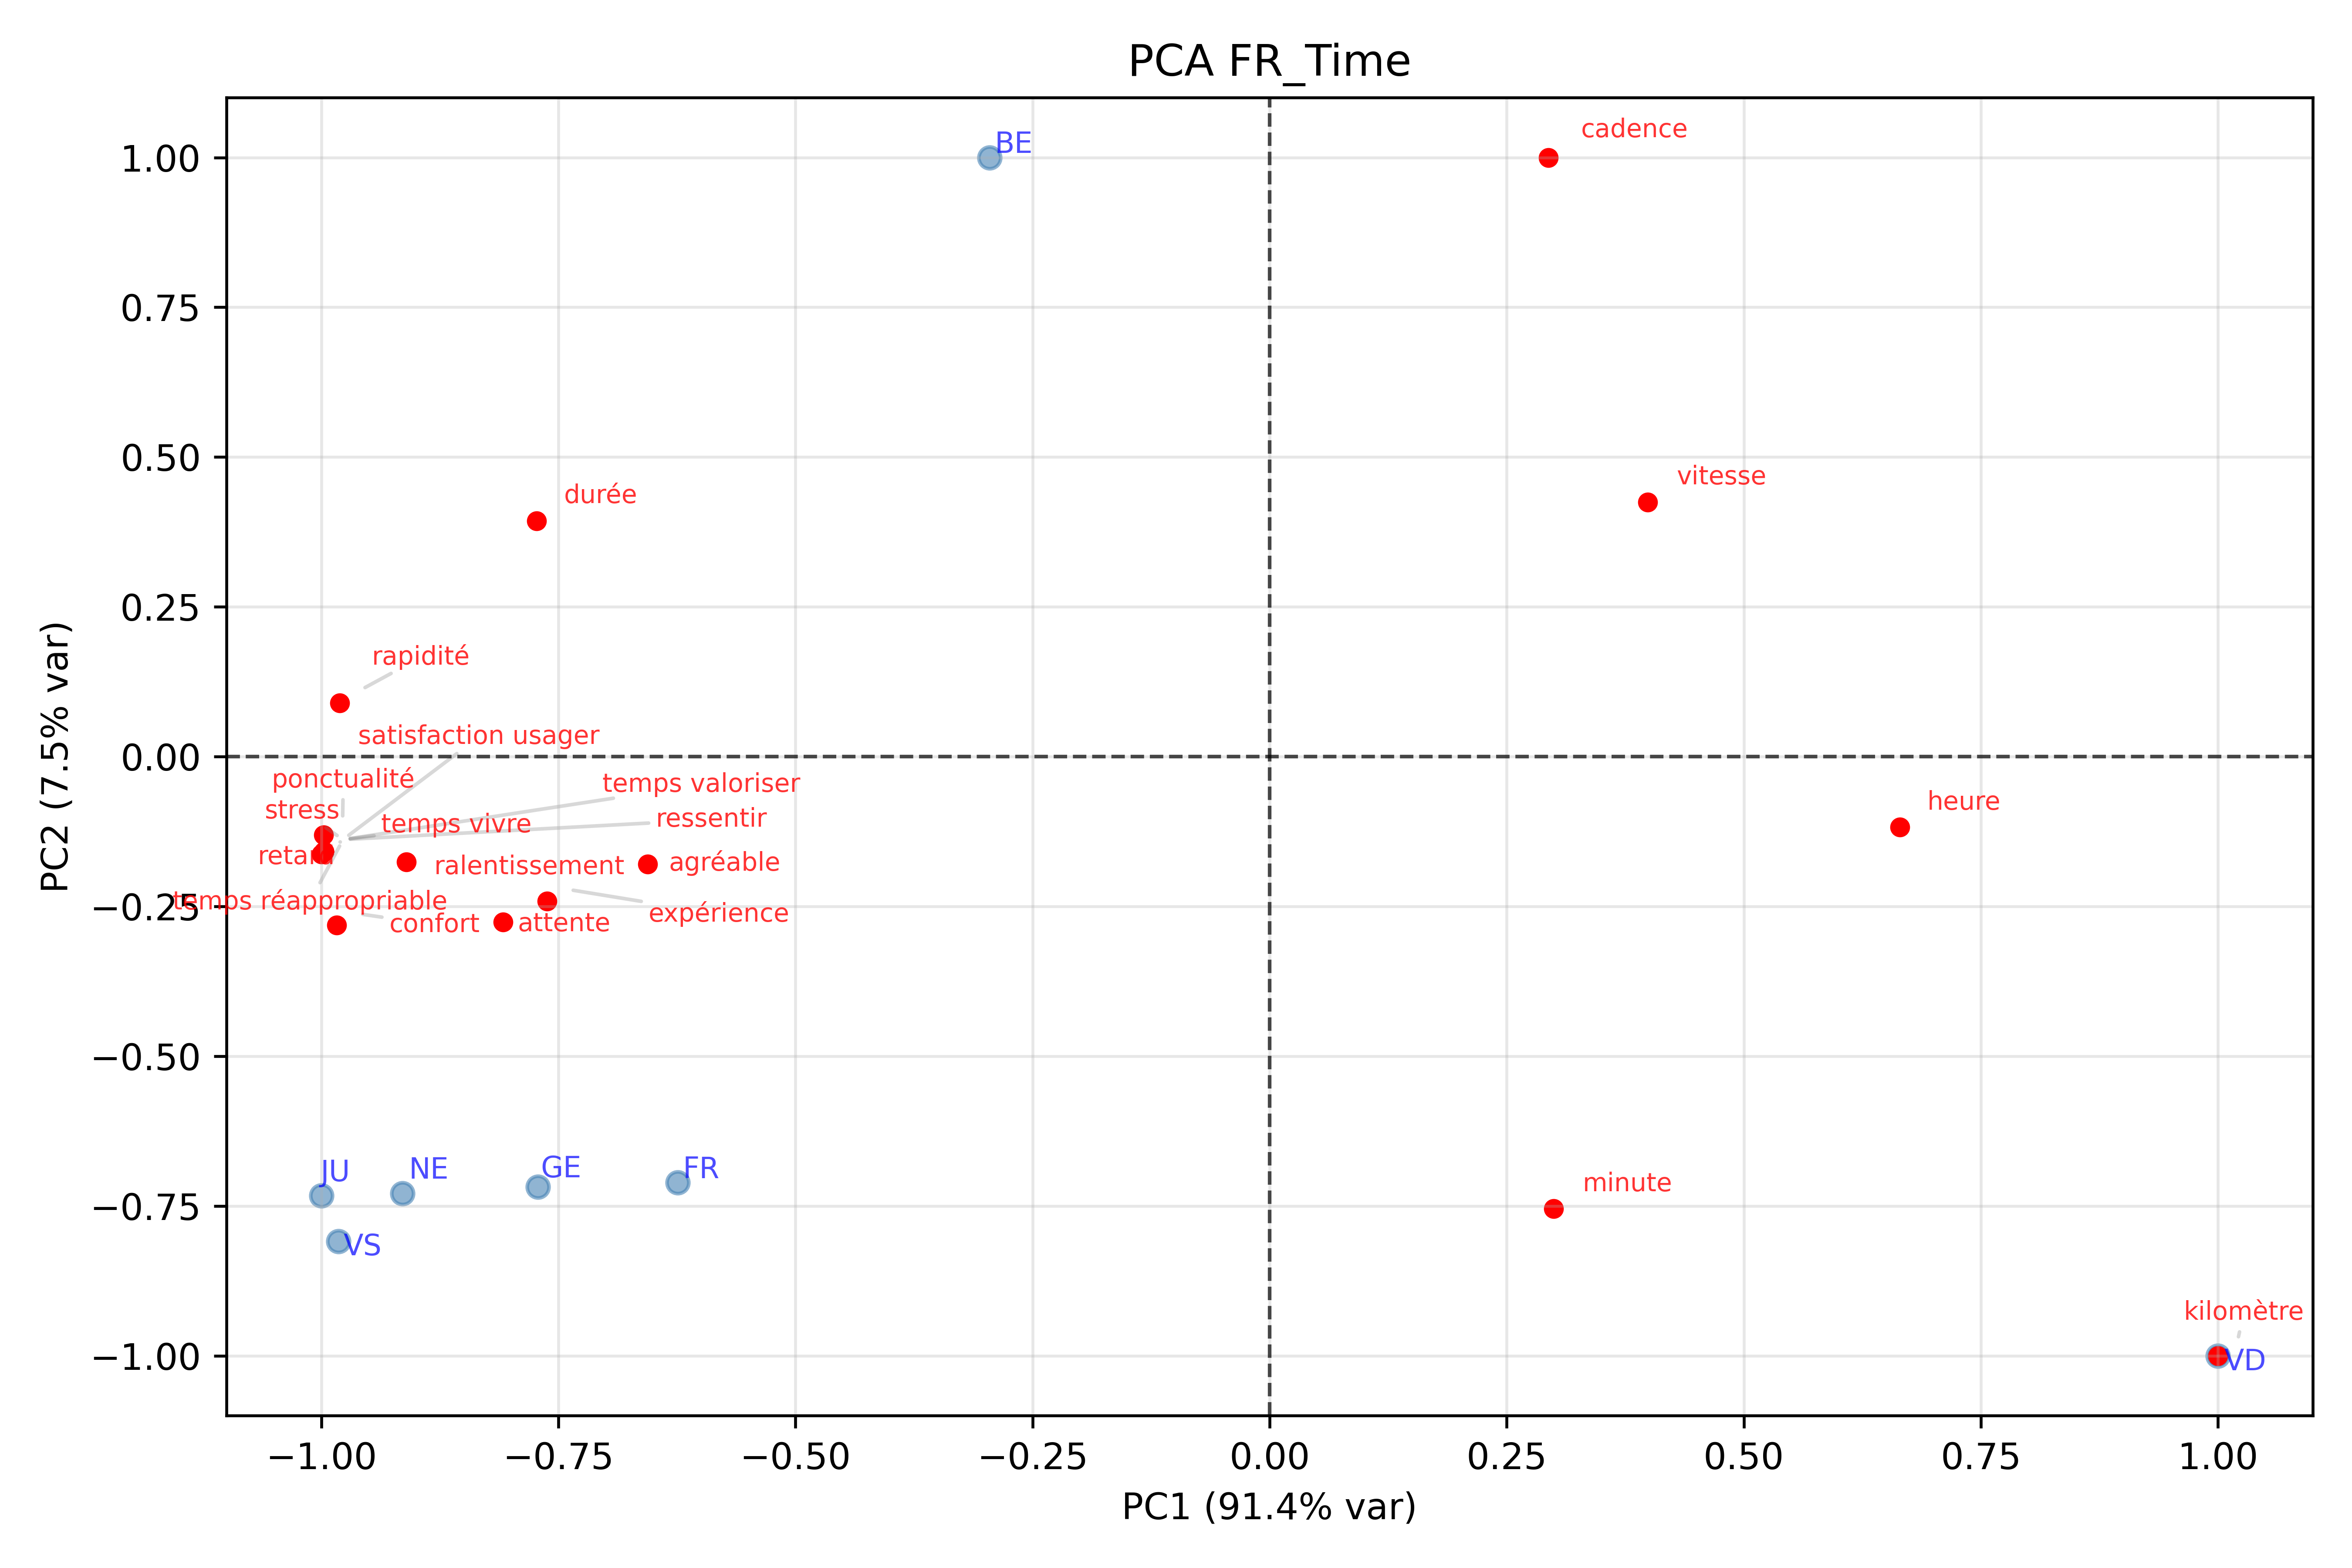
\includegraphics[width=0.95\linewidth]{Analysis/software/result/PCA_FR_Time.png}
    \caption{\textit{The French PCA highlights the dominance of quantifiable temporal notions, while 
subjective or experiential terms remain marginal in their contribution to variance.}}
    \label{fig:PCA_FR_time}
\end{figure}

\begin{figure}[H]
    \centering
    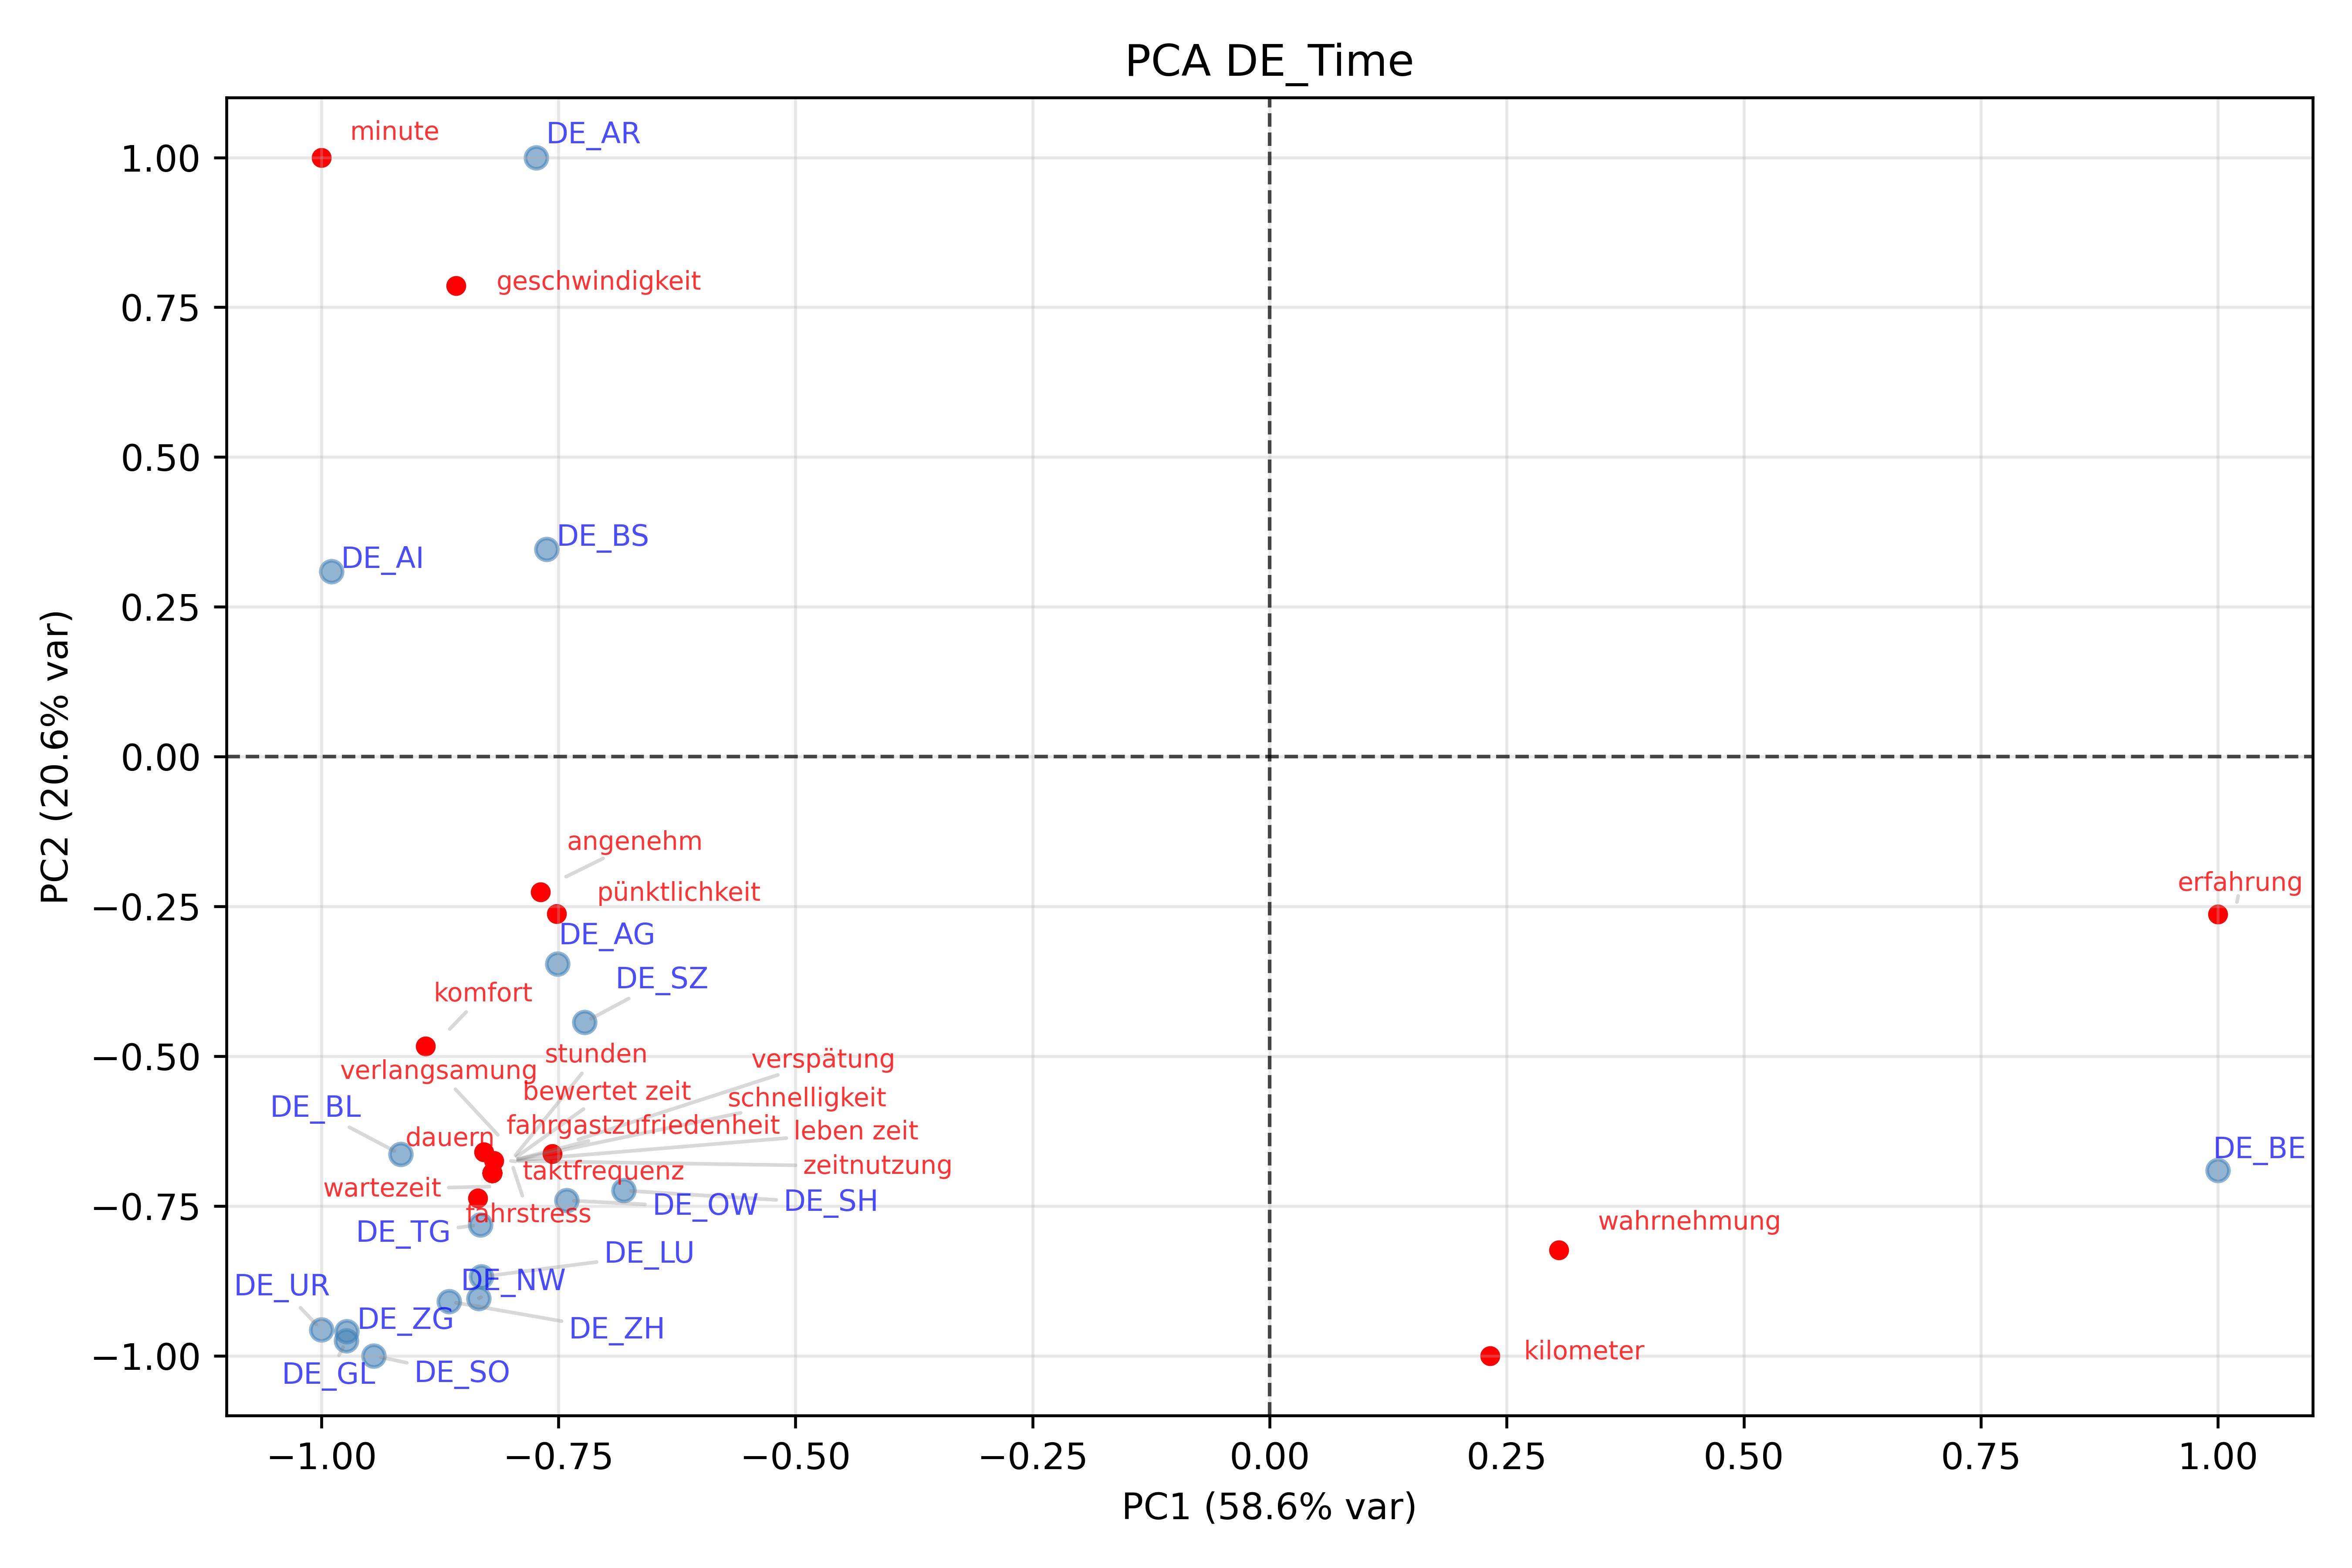
\includegraphics[width=0.95\linewidth]{Analysis/software/result/PCA_DE_Time.png}
    \caption{The German PCA confirms the strong prevalence of measurable time markers, with 
experiential notions appearing peripheral and weakly structuring the corpus.}
    \label{fig:PCA_DE_time}
\end{figure}

\newpage

\subsection{Analysis of PCA Results related to mobility}

Figure~\ref{fig:PCA_FR_mobility} shows a clear opposition between highly operational 
mobility notions and more capability-oriented terms. The first principal component captures the strong weight of "infrastructure", which dominates the positive side of the axis and forms the main structuring force in the corpus along with "coût", "accessibilité", "réseau transport" and "qualité desserte". 
Experiential or capability-related notions like "motivation mobilité", "apprentissage 
mobilité" or "habitus mobilité" cluster on the left very tightly together, indicating that they co-vary as a group but contribute only weakly to structuring differences between documents. The 
cantonal documents form a dense cluster near the negative side of the horizontal axis, except for Vaud and Bern, which are isolated at the positive extreme, similarly to the time PCA. This position suggests that VD relies more heavily 
on infrastructure and technical vocabulary than other French-speaking cantons, which 
use capability-based terms even more rarely than the others.

As shown in Figure~\ref{fig:PCA_DE_mobility}, the German corpus displays a similar 
structure, with "infrastruktur" and "kosten" anchoring opposite sides of the second 
principal component. Capability-related terms such as "mobilitätskompetenz", 
"bewegungsautonomie" or "mobilitätshabitus" cluster near the centre and form a dense 
semantic block. Their central position indicates that they vary little across the 
documents and are very underrepresented per table \ref{table:table_motility}; they are not the primary drivers of separation. The cantons again cluster 
tightly on the negative side of the horizontal axis, with BS, BL and BE positioned at the two extremes of the first two components. 
These outliers reflect a stronger emphasis on specific operational themes in these 
cantons, while the rest of the German-speaking corpus remains lexically homogeneous. 
Overall, measurable and infrastructural notions structure the corpus far more strongly 
than capability-related vocabulary.


\begin{figure}[H]
    \centering
    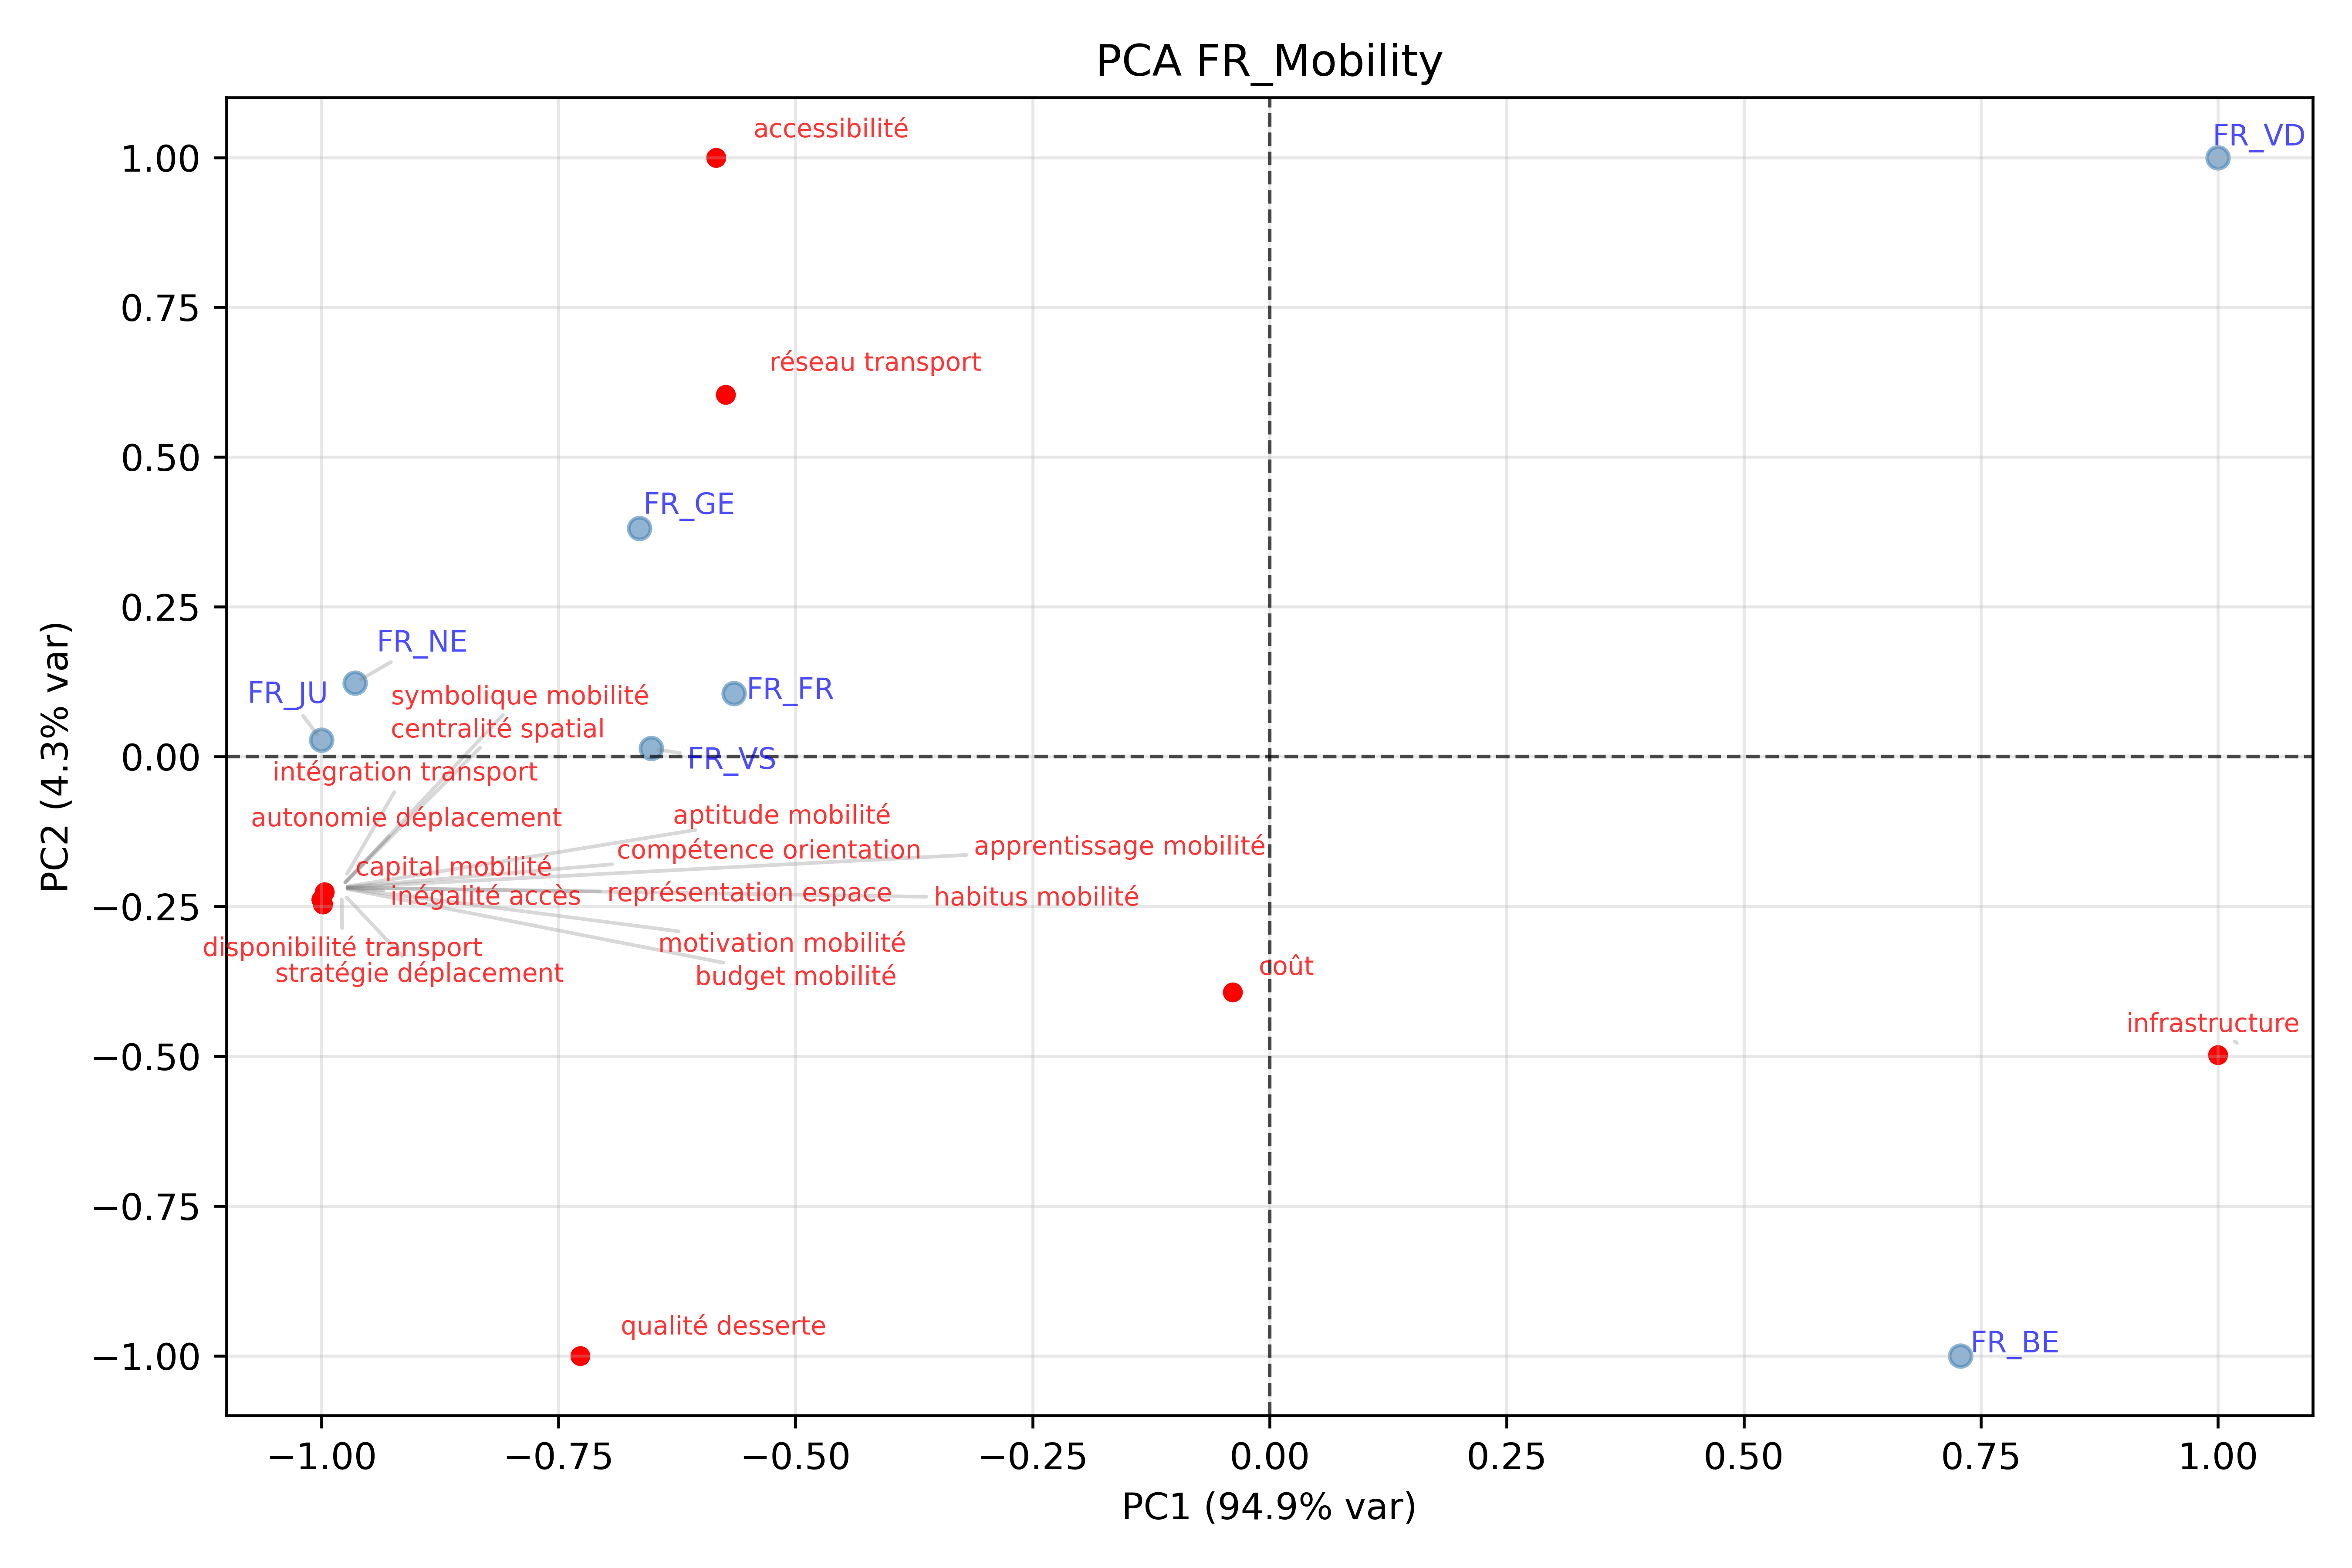
\includegraphics[width=0.95\linewidth]{Analysis/software/result/PCA_FR_Mobility.png}
    \caption{The French PCA reveals a strong axis contrasting infrastructure-focused terms with 
capability-oriented mobility notions, with VD standing apart from the other cantons.}
    \label{fig:PCA_FR_mobility}
\end{figure}

\begin{figure}[H]
    \centering
    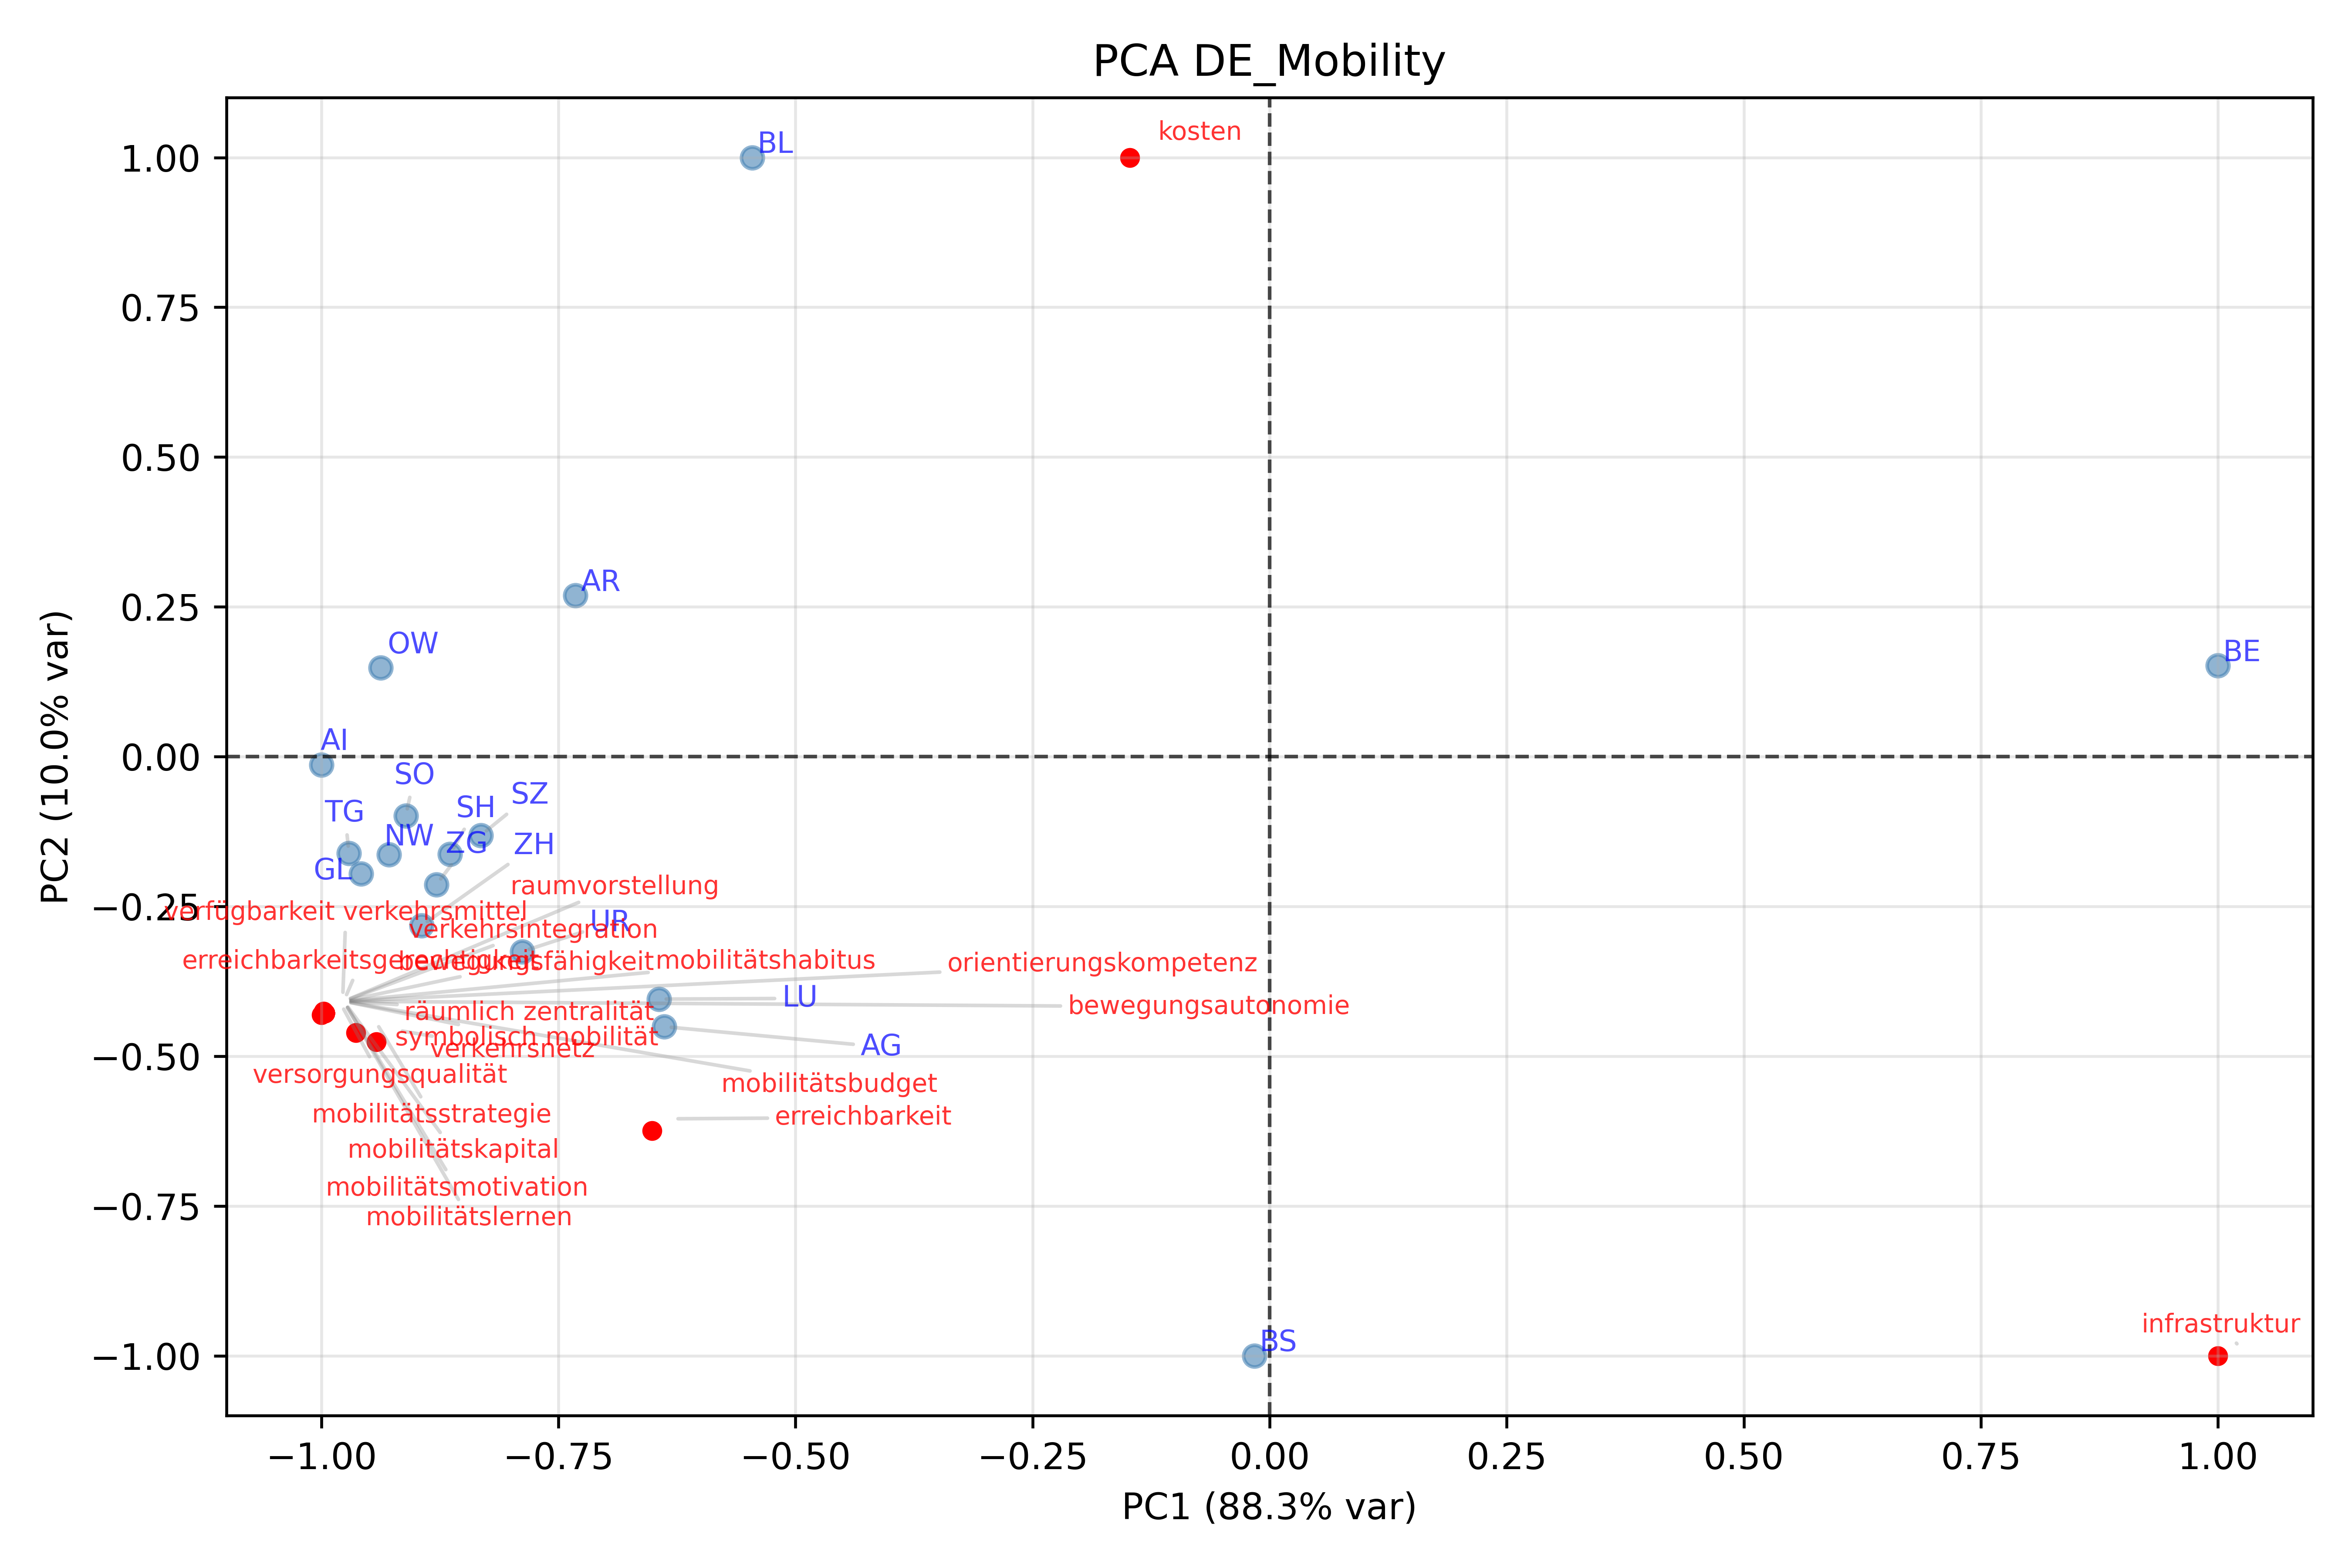
\includegraphics[width=0.95\linewidth]{Analysis/software/result/PCA_DE_Mobility.png}
    \caption{The German PCA highlights the dominance of operational and infrastructural mobility 
terms, while capability-related notions remain central and weakly discriminant.}
    \label{fig:PCA_DE_mobility}
\end{figure}

\subsection{Synthesis}

Combining the AFC results with the word occurrence analysis reveals a coherent narrative: Swiss spatial planning discourse is heavily skewed toward measurable, supply-oriented dimensions of mobility. Accessibility and physical time terms dominate both corpora, while motility and subjective time concepts are almost absent. This is consistent across French and German texts. 

Motility is conceptually underrepresented, indicating that planners primarily consider mobility as a function of infrastructure, services, and network performance rather than individual capabilities, skills or motivation. Time is similarly treated as a quantifiable variable, with minimal attention to comfort, perception or human experience. 

The combined word frequency and AFC results reinforce the conclusion that Swiss planning documents operationalize mobility and time in terms of provision and efficiency. Human-centered aspects, including cognitive, motivational and experiential dimensions, remain peripheral, reflecting a narrow and infrastructure-focused view of mobility.

\section{Discussion}
Limitation of the keyword approach
need to either Analyse factoriel exploratoire / confirmatoire pour montrer que les listes de mots matchent bien avec le concept latent. 

talk about implication of our result
\section{Conclusion}

This study examined how accessibility, motility, and time are represented in Swiss spatial planning discourse using a textometric approach. The analysis reveals a clear imbalance in planning language. Accessibility is widely present and discussed in concrete terms, whereas motility, which encompasses skills, motivation, and cognitive appropriation, is almost entirely absent. This absence indicates that capability-based dimensions of mobility are not yet part of the institutional vocabulary, making them difficult to plan for or evaluate.

Time is represented asymmetrically as well. References to physical and objective time appear frequently and are treated as operational variables to be measured or minimized. Perceived or subjective time appears to a lesser extent. Concepts such as comfort are mentioned but remain vague and underdeveloped. This suggests that planners have begun to acknowledge experiential aspects of travel, yet they do not articulate them in operational terms.

Methodologically, the textometric pipeline proved effective at revealing patterns of presence and absence in institutional language. It is valuable for mapping what planning discourse renders thinkable and actionable. At the same time, the approach is essentially descriptive. Combining it with contextual and semantic analyses would better recover meaning beyond raw counts, reducing reliance on manual interpretation and mitigating researcher bias.

The project’s contributions are twofold. First, it documents a persistent discursive bias in official planning documents toward supply-side and technical framings of mobility. Second, it provides a reproducible dataset and analysis pipeline, released under a CC-BY license in the project repository \cite{morand_nathmoswissspatialplanningtextometricanalysis_2025}, enabling further research or replication. Making this corpus freely available lowers the "cost" of entry and allows exploration of broader aspects of spatial planning beyond mobility alone.

Looking forward, bridging the gap between accessibility and motility requires both conceptual and institutional change. We need ways to measure motility without oversimplifying it, and planning should routinely collect data on experiential and behavioral dimensions without falling into's Goodhart's law. Only then can mobility policy move beyond networks to truly support people’s capabilities and maybe let the author sleep a little easier knowing that Switzerland point a bit more toward a sustainable future.
\section{Appendix}

\subsection{logbook}

\begin{itemize}[leftmargin=1.5cm,label={}]
    \item[\textbf{2025-08-27}] kickoff meeting
    \item[\textbf{2025-09-13}] Mooc textometrie, recherche des sources de document
    \item[\textbf{2025-09-15}] Investigation de la structure entre les documents, Formation du Dataset
    \item[\textbf{2025-09-25}] Creation of this report, rough layout of the idea in chapter + meeting with supervisor
    \item[\textbf{2025-10-02}] Formation recherche Zotero
    \item[\textbf{2025-10-05}] Définition du champ l'exical en rapport aux questions de recherche, Analysis in TXM, searching for patterns
    \item[\textbf{2025-10-15}] Presentation mis semestre kaufmann + Jules
    \item[\textbf{2025-10-16}] Script python, run against word list
    \item[\textbf{2025-10-16}] Made motilité word list
    \item[\textbf{2025-10-22}] Made german list + analysis, sent email for previous version
    \item[\textbf{2025-10-24}] Writing
    \item[\textbf{2025-10-26}] Sorting PDF + AFC setup using TXM (failure)
    \item[\textbf{2025-10-27}] Writing, re-run analysis with new document
    \item[\textbf{2025-10-28}] finished new script to make clean AFC in python
    \item[\textbf{2025-10-29}] added one more document received by email, writing methodology
    \item[\textbf{2025-11-07}] Visio avec Thomas Bühler
    \item[\textbf{2025-11-10}] rework AFC + wordlist
    \item[\textbf{2025-11-17}] analysis, result writing
\end{itemize}

\subsection{scripts}

\begin{lstlisting}[caption={Extract text content from PDFs by language}, label={lst:extract_pdfs}]

mkdir -p ../TXT && for f in *.pdf; do lang="${f:0:2}";
mkdir -p "../TXT/$lang";
pdftotext "$f" "../TXT/$lang/${f%.pdf}.txt"; done

\end{lstlisting}


% Add appendices here, if there are any

\newpage
\bibliographystyle{plainurl} 
\bibliography{References}

\end{document}
